\documentclass[%
 aps,
 pra,
 longbibliography,
 amsmath,amssymb,
 reprint,
 superscriptaddress,
 %groupedaddress,
]{revtex4-1}

\usepackage{graphicx}
\usepackage{epstopdf}
\usepackage{natbib}
\usepackage{bm}


\begin{document}

\title[Reversible mechanical and electrical properties of ripped graphene]{Reversible mechanical and electrical properties of ripped graphene}

\author{J. Henry Hinnefeld}
 \affiliation{Department of Physics, University of Illinois at Urbana-Champaign, 1110 West Green Street, Urbana, Illinois 61801, USA}
\author{Stephen T. Gill}
 \affiliation{Department of Physics, University of Illinois at Urbana-Champaign, 1110 West Green Street, Urbana, Illinois 61801, USA}
\author{Shuze Zhu}
 \affiliation{Department of Mechanical Engineering, University of Maryland, College Park, MD 20742, USA}
\author{William J. Swanson}
 \affiliation{Department of Physics, University of Illinois at Urbana-Champaign, 1110 West Green Street, Urbana, Illinois 61801, USA}
\author{Teng Li}
 \affiliation{Department of Mechanical Engineering, University of Maryland, College Park, MD 20742, USA}
\author{Nadya Mason}
 \email{nadya@illinois.edu}
 \affiliation{Department of Physics, University of Illinois at Urbana-Champaign, 1110 West Green Street, Urbana, Illinois 61801, USA}

\date{\today}

\begin{abstract}
We examine the mechanical properties of graphene devices stretched on flexible
elastomer substrates. Using atomic force microscopy, electrical transport
measurements, and mechanics simulations, we show that micro-rips form in the
graphene during the initial application of tensile strain; however subsequent
applications of the same tensile strain elastically open and close the existing
rips. Correspondingly, while the initial tensile strain degrades the devices'
transport properties, subsequent strain-relaxation cycles affect transport only
moderately, and in a largely reversible fashion, yielding robust electrical
transport even after partial mechanical failure. Graphene's combination of
superlative electronic properties, extreme flexibility, and robust
functionality after partial mechanical failure is unique among conducting thin
films and lends itself to a variety of promising future device applications;
the new understanding provided here of when and how graphene rips can directly
impact the design of novel graphene-based devices which are required to
function under strain.
\end{abstract}

\maketitle

\section{Introduction}

Recent advances in graphene production\cite{Kim2009, Bae2010, Lee2010} have
enabled the fabrication of a variety of flexible, graphene-based electronic
components, including transparent interconnects\cite{Kim2011}, high-performance
capacitors\cite{El-Kady2012}, and transistors\cite{Lee2011}. The prospect of
flexible and transparent graphene-based electronic devices suggested by these
results raises an important question: are graphene's electrical properties and
mechanical integrity robust under the strains graphene is likely to experience
in such devices? Pristine graphene has an exceptionally high breaking
strength\cite{Lee2008}, yet it may be susceptible to ripping, particularly if
it has defects \cite{Kim2012} and/or strong  surface adhesion\cite{Sen2010}. It
is still relatively unknown under what strain conditions substrate-supported
graphene rips, and how the electrical properties are then altered.

In this manuscript, we combine atomic force microscopy (AFM), coarse-grained
mechanical simulations, and electrical transport measurements to study the
effects of lateral strain on rips in graphene. We find that graphene adhered to
a flexible substrate and then stretched laterally can develop small rips with
only 1\% applied strain. However, even with ripping, the electrical properties
remain relatively robust: introducing small rips slightly increases the
resistance, but subsequent strain-relaxation cycles over the same strain range
change transport only modestly, and in a largely reversible fashion. Such
resilience is atypical for conducting thin films, which typically demonstrate
rapid and irreversible device failure after the onset of rip
formation\cite{Cairns2000,Fortunato2002}.

\begin{figure}[floatfix]
\centering
\vspace{0.2cm}
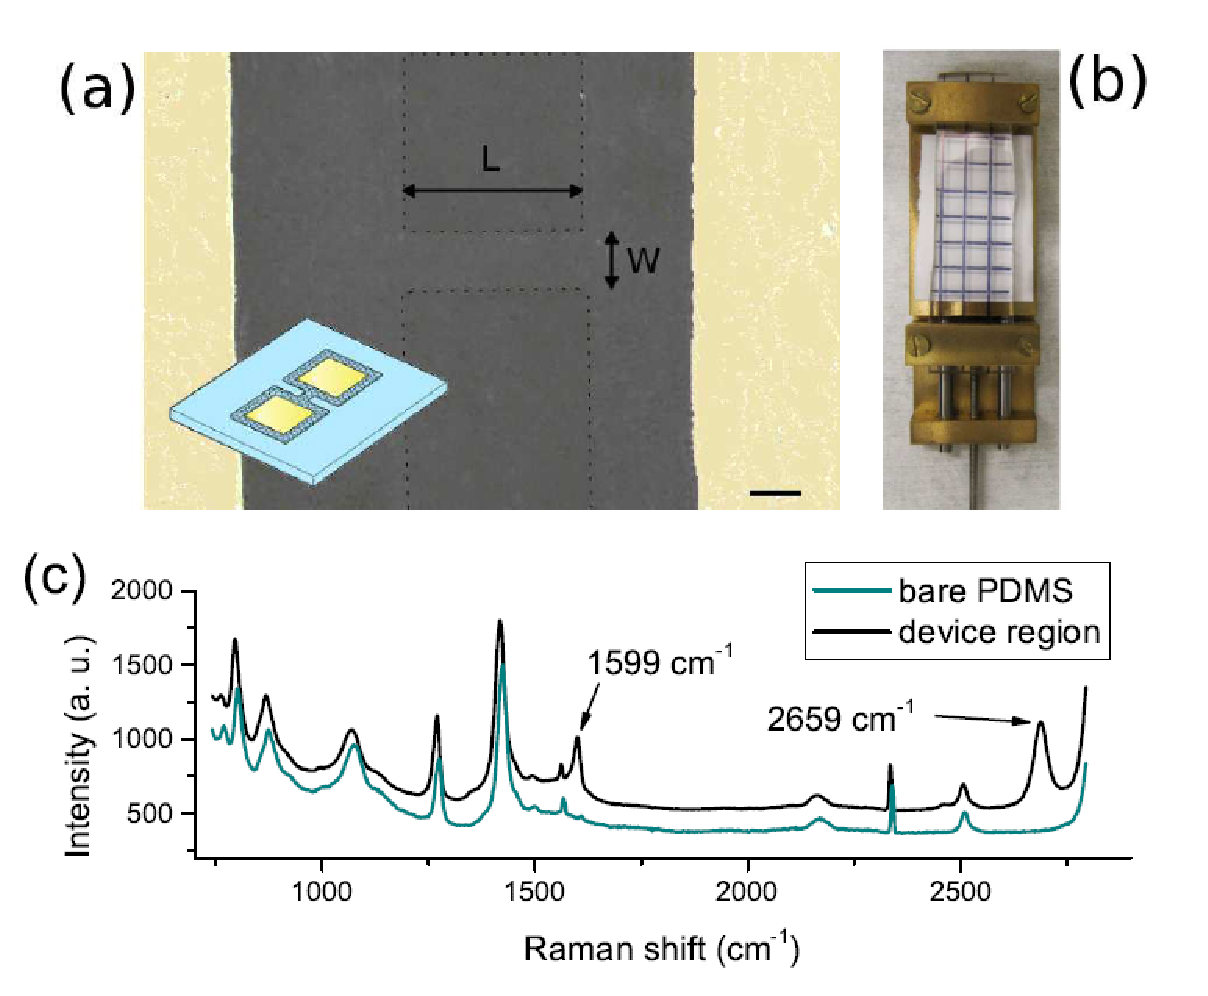
\includegraphics[width=\linewidth]{Figure1.eps}
\caption{\textbf{(a)} False-color optical image of a graphene bridge device
    (outlined by dashed line) patterned on a PDMS substrate with gold contact pads
    (light yellow). The length (L) and width (W) of the bridge are described in the
    text. The scale bar is 25 $\mu$m. Inset: A schematic illustration of the device
    geometry. \textbf{(b)}  The mechanical stretching stage with PDMS inserted
    between the clamps. The devices are stretched along the axis of the
    micro-bridge. \textbf{(c)} Offset Raman spectra for a bare PDMS region and a
    graphene device region. The graphene G and 2D peaks, at 1599 cm$^{-1}$ and 2659
    cm$^{-1}$ respectively, in the spectra from the device region confirm the
    presence of graphene.}
\label{fig:device}
\end{figure}

This new understanding of when and how graphene rips, and how its electrical
properties are thereby altered is immediately applicable to the implementation
and production of devices which include the graphene-based components mentioned
above. Some applications, for instance frequency-tuned RC circuits using
graphene capacitors and interconnects, would require careful consideration of
what strains the device can withstand while keeping strain-induced variations
in the electronic properties of graphene within the required specifications.
Likewise, in applications such as portable consumer electronics where low power
consumption is a priority the increased resistance of strained graphene films
may limit the potentially applicable strain, or require the use of more
complicated interconnect geometries\cite{Kim2011}. Graphene's exceptional
resilience as described here may also motivate its inclusion in device
applications where other conducting thin films have been used to date;
bio-integrated devices\cite{Viventi2010} are especially appealing candidates
because of the difficulty involved in replacing devices installed \textit{in
vivo}, as well as because of graphene's non-toxicity.

\begin{figure*}
\centering
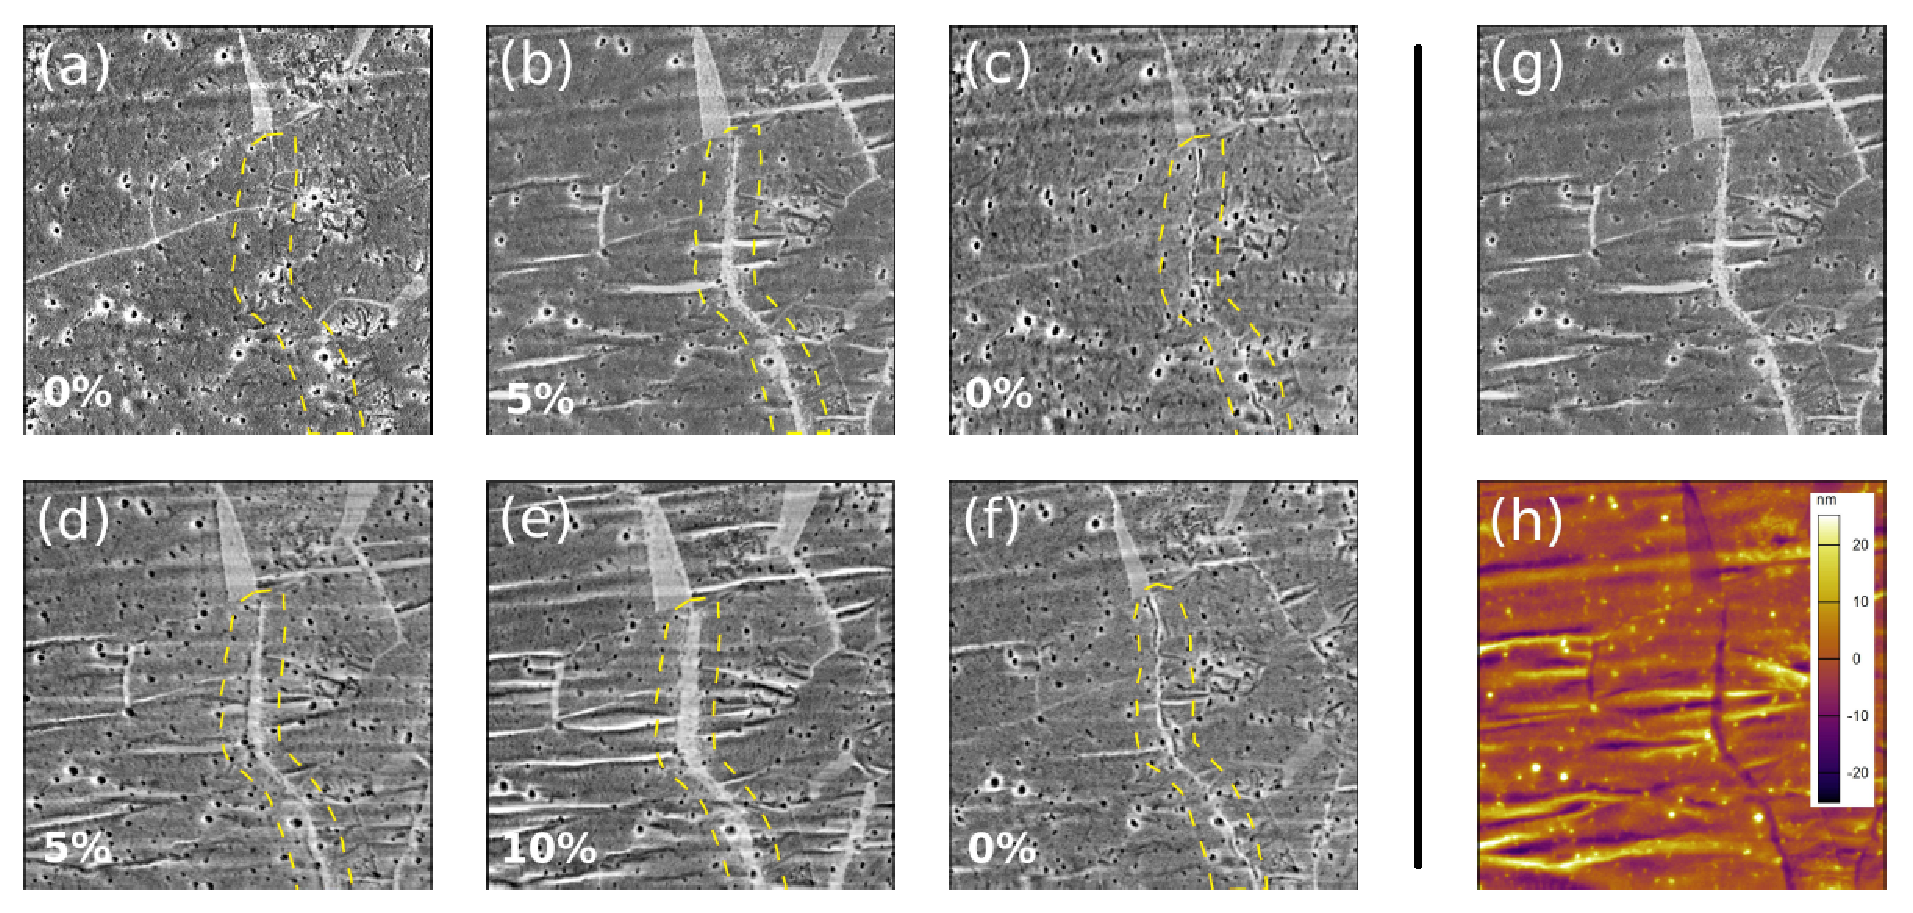
\includegraphics[width=\linewidth]{Figure3.eps}
\caption{\textbf{(a-f)} AFM phase measurements of graphene on a polymer
    substrate at approximately 0, 5, 0, 5, 10, and 0 percent strain (applied along
    the horizontal axis), as labeled. Rips are evident as light-gray, elongated
    vertical features. An example of a rip that opens and closes with applied
    strain is indicated by the dashed line. Dark spots present in each image are
    debris on the substrate surface; white halos surrounding some of the debris are
    indicative of graphene slightly delaminating from the substrate. Elongated
    horizontal features are strain-dependent wrinkles. \textbf{(g)} AFM phase and
    \textbf{(h)} height data. Variations in the height data distinguish between
    wrinkles and rips in the graphene, which have similar signatures in the phase
    data. The scanned area in each image is 25 $\mu$m$^2$.}
\label{fig:rips}
\end{figure*}

\begin{figure}
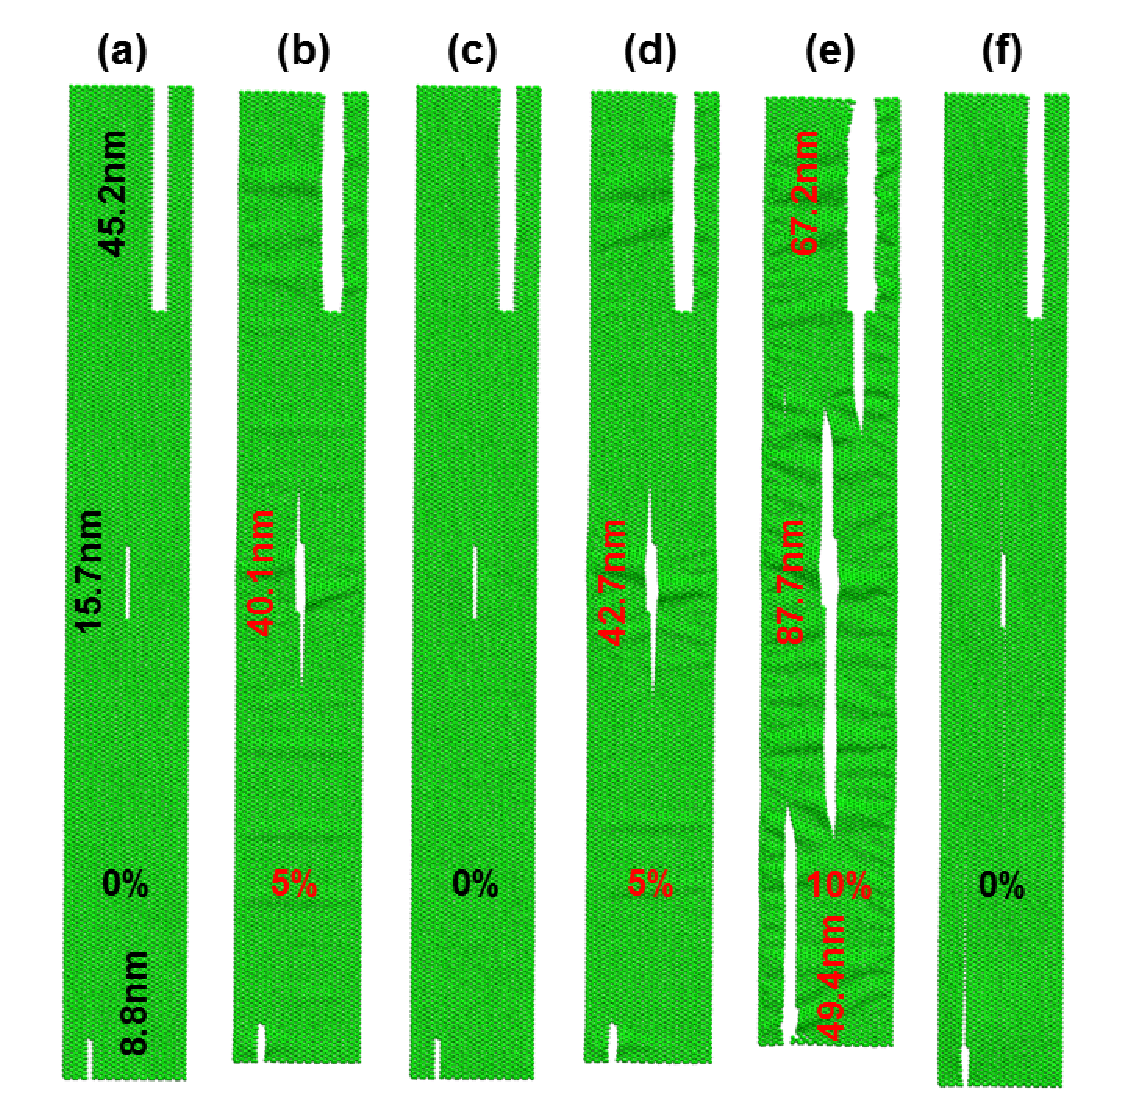
\includegraphics[width=\linewidth]{Figure4.eps}
\caption{Coarse-grained simulations show the elastic opening and closing of
    rips during initial and subsequent tensile loading cycles, in good agreement
    with AFM measurements in Figure 2. The graphene region was simulated at 0, 5,
    0, 5, 10, and 0 percent strain applied along the horizontal axis, as labeled.
    Values given in nm refer to the rip lengths. The vertical contraction of the
    graphene region at higher strain values is due to the Poisson effect.}
\label{fig:Simulation}
\end{figure}

\begin{figure*}
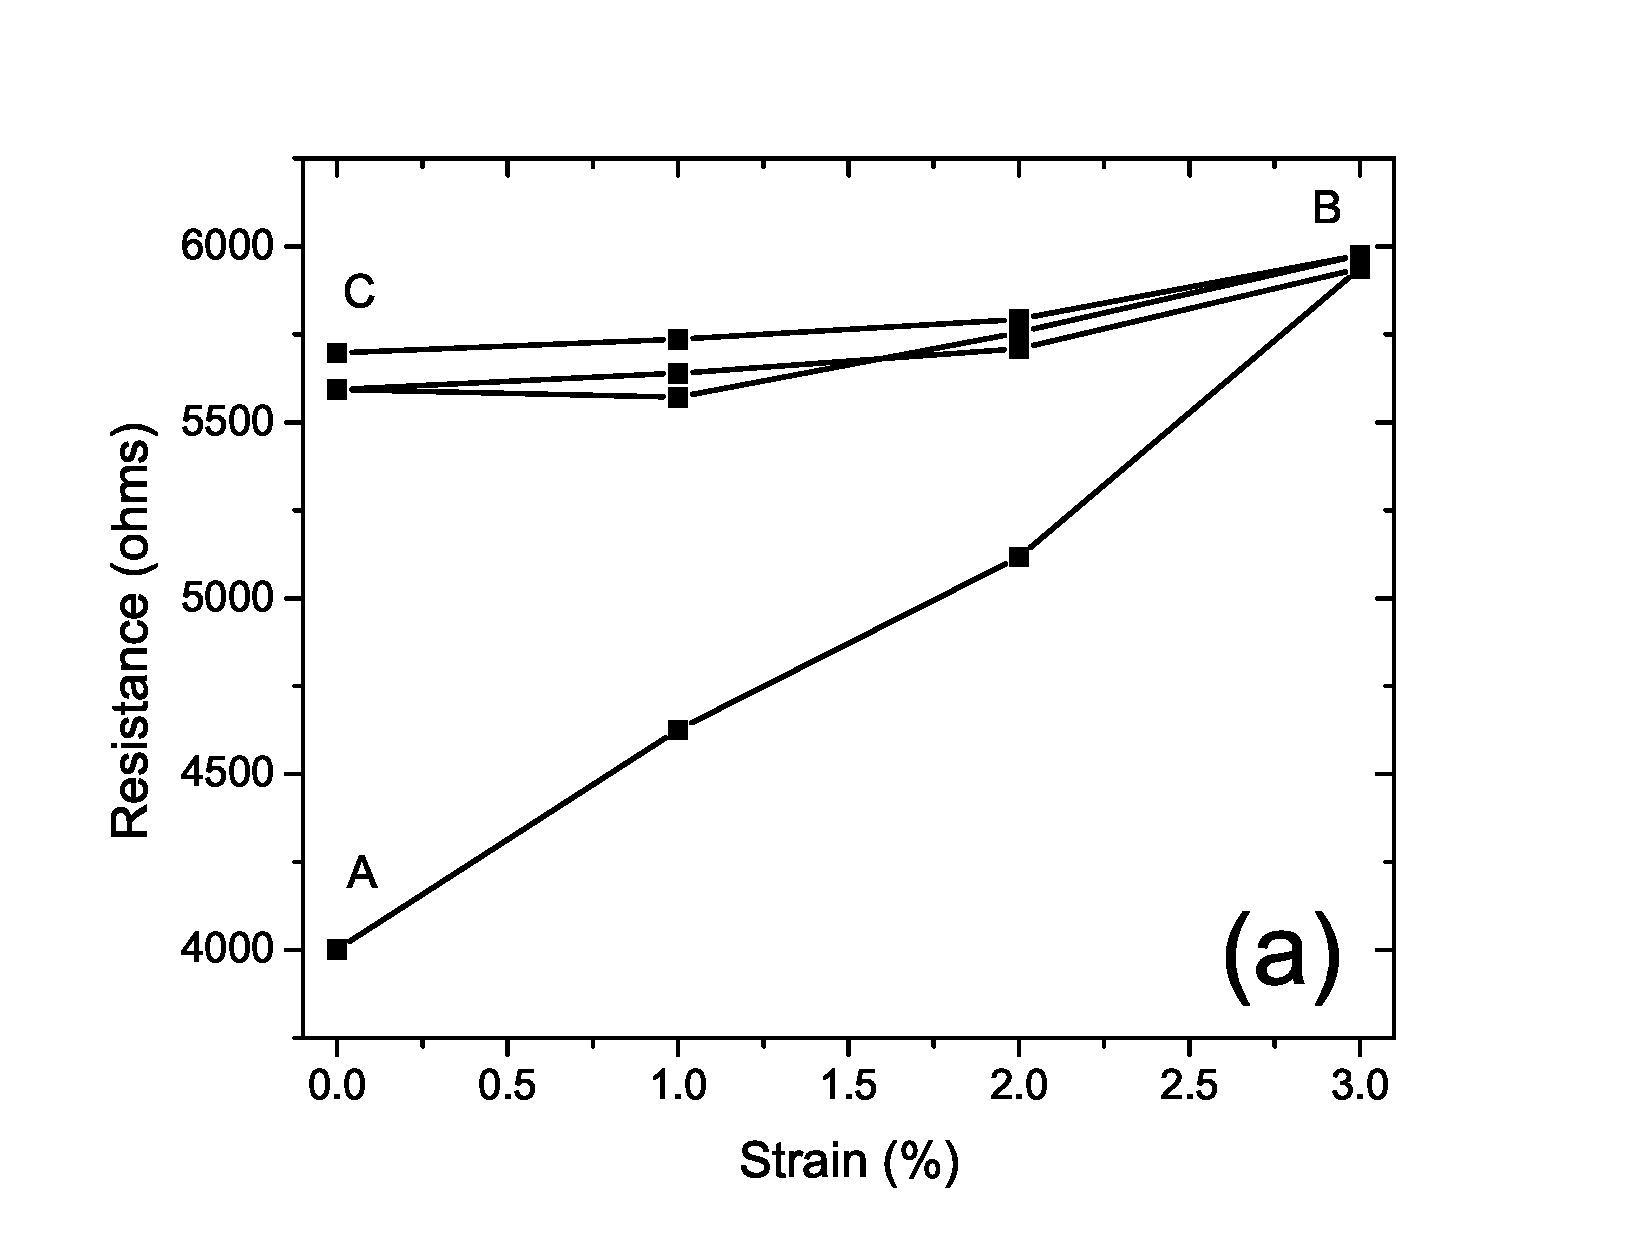
\includegraphics[width=0.49\linewidth]{Fig2a.eps}
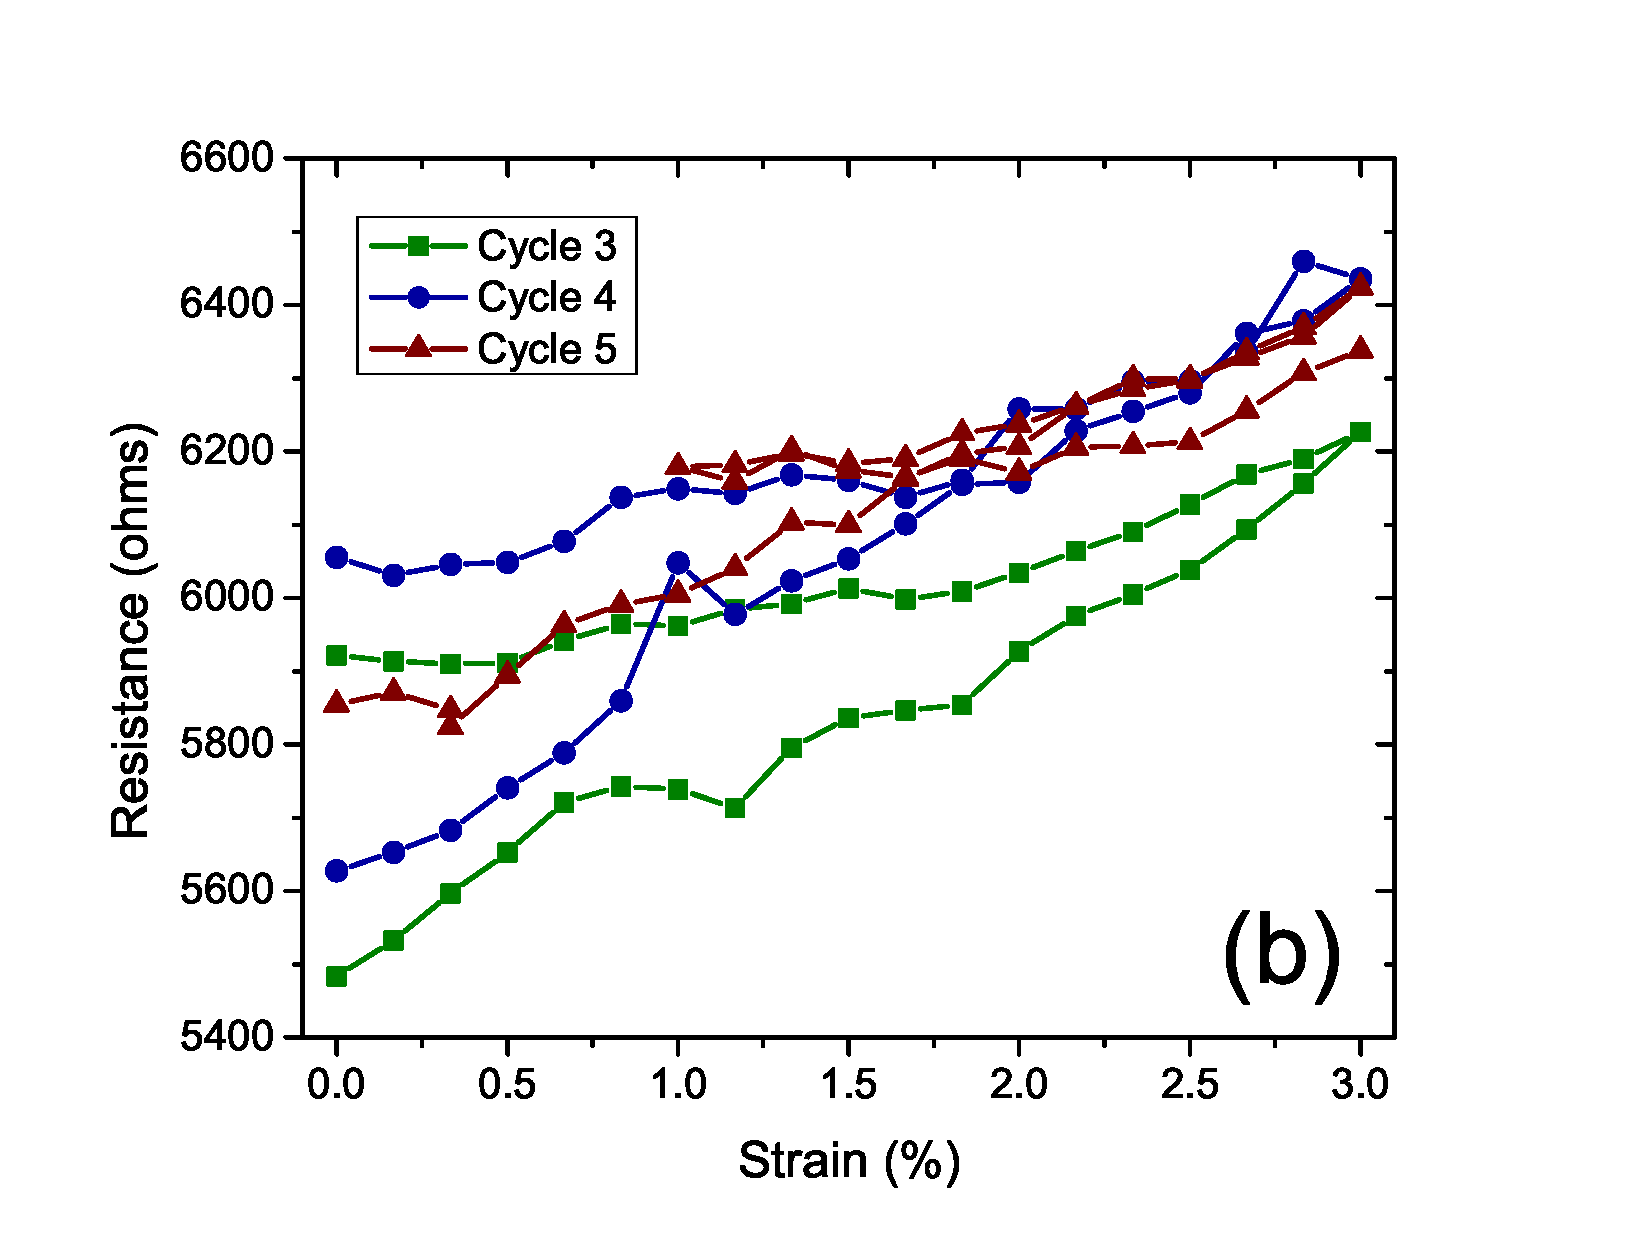
\includegraphics[width=0.49\linewidth]{Fig2b.eps}
\caption{\textbf{(a)} Electrical resistance of a graphene device vs. applied
    tensile strain. The initial application of strain significantly increases the
    resistance while subsequent strain-relaxation cycles over the same strain range
    yield smaller, mostly reversible changes in the resistance. \textbf{(b)} Three
    consecutive strain-relaxation cycles (Cycles 3,4,5), showing largely reversible
    transport characteristics.}
\label{fig:RvsStrain}
\end{figure*}



\section{Experimental Details}

Devices consisted of patterned graphene placed on flexible polydimethylsiloxane
(PDMS) substrates. The devices were fabricated using a modified transfer
printing process, similar to that described in Ref \onlinecite{Kim2009}.
Single-layer graphene was grown using established chemical vapor deposition
(CVD) techniques \cite{Li2009}, and then transferred to a copper-coated silicon
wafer where it was patterned using photolithography and reactive ion etching.
Next, a piece of PDMS was mechanically pressed onto the silicon wafer, and the
copper was then etched to leave patterned graphene on the PDMS
substrate\cite{Lee2010}. Raman spectroscopy was used to confirm the presence of
graphene on the PDMS as shown in Figure 1c; the shape of the Raman 2D
peak\cite{Ferrari2006}, as well as subsequent AFM measurements verified the
single-layer character of the graphene. Finally, shadow-mask evaporation was
used to deposit Ti/Au contact pads. The device geometry is illustrated in
Figure 1a: a narrow graphene bridge connects two large graphene pads, each of
which is covered with a Ti/Au contact pad. We studied 13 different devices
having bridge aspect ratios ranging from 1.5:1 to 12:1 (length:width) and
widths of 100, 50, and 25 $\mu$m. The data in this manuscript focuses on a
device with a bridge width of 25 $\mu$m and an aspect ratio of 2:1. The data
for all samples yielded similar qualitative results. Quantitative differences
in transport data between different devices were uncorrelated with the bridge
dimensions, and instead seemed to be dominated by pre-existing rips in the
graphene, which are often introduced during the graphene transfer
process\cite{Kim2012}.

AFM and transport measurements were performed while the PDMS substrate was
mounted in a mechanical stretching stage, as shown in Figure 1b. The substrate
was clamped at either end, and then strained by turning the threaded rod, which
laterally moves the sliding clamp along its guide rails. A mechanical stepper
motor was used to control the stretching stage position to ensure
reproducibility. Variable device positioning on the substrate as well as slight
variations in substrate thickness preclude exact conversion between strain
applied to the substrate and to the device, therefore `turns of the stretching
stage control rod' were used as the controlled variable. Each turn strains the
substrate by approximately one percent, and we estimate that the strain applied
to the graphene differs from that applied to the PDMS substrate by no more than
ten percent. However, our conclusions are unaffected by this uncertainty, as
variations in the magnitude of applied strain between devices only shift the
strain axis of the data while preserving the observed trends. Optical
observations indicated that the Ti/Au pad adhesion to the substrate was robust
and did not slip during measurements. Transport measurements were performed by
placing micro-manipulator probes in contact with the gold contact pads at each
strain value, and AFM measurements were performed with an Asylum Research
MFP-3D.

\section{Results and Discussion}

\subsection{Topology of Rips}
Figures 2a-f show AFM phase images of graphene in the bridge region of a device
at 0, 5, 0, 5, 10, and 0 percent strain applied along the horizontal axis of
the images. Both rips and delaminations caused by wrinkles appear as a function
of strain, and can be distinguished via AFM height data: Figs. 2g and 2h show
that wrinkles have corresponding undulations in the height data (peaks and
dips) while rips are indicated by a uniform depression (consistent with the
substrate exposed between graphene regions). In Fig. 2, the vertical features
are rips and the majority of the horizontal features are wrinkles.

The opening and closing of rips is clear in the Figure:  the unstrained device
(Fig. 2a) exhibits some small rips and defects. When the substrate is
mechanically stretched (Fig. 2b) the existing rips widen and new rips form;
when the applied strain is relaxed (Fig. 2c), pre-existing defects return to
nearly their original condition and newly formed rips close. Subsequent
strain-relaxation cycles over the same strain range re-open existing rips (Fig.
2d), but proceeding to a higher strain range forms new rips and widens
pre-existing ones (Fig. 2e), which then close less completely when the strain
is relaxed (Fig. 2f). The strain values at which we observe micro-rip formation
are substantially lower than the reported fracture strength of
graphene\cite{Lee2008}, however the tensile strength of graphene is strongly
susceptible to defects such as holes and tears\cite{Lee2013}. Although graphene
produced by CVD is known to be polydomain, it has been shown that rips in
graphene do not preferentially follow grain boundaries\cite{Kim2012}. Rather,
the fabrication procedures used to generate patterned graphene devices on
polymer substrates routinely introduce rips and other defects in the graphene,
which accounts for the mechanical failure observed at low strain values.

\subsection{Simulation of Rip Formation}
To shed light on the underlying mechanism of the rip formation and evolution,
we simulate rip formation and the subsequent elastic opening and closing of
rips in graphene, via a coarse-grained (CG) modeling scheme\cite{Zhu2014}.
Given the prohibitive simulation expense to model rips of real size in
experiments (microns in length), we simulate a scaled-down model of a graphene
monolayer with a size of 24 nm by 200 nm (Fig. 3). Three pre-cracks of various
sizes are introduced in the model (Fig. 3a) to mimic the pre-existing defects
in the as-made sample. Each CG bead in the graphene interacts with a virtual
substrate via a Lennard-Jones potential\cite{Scharfenberg2011} $V_{gs}(r)
=4\varepsilon_{gs} \left( \frac{\sigma_{gs}^{12}}{r^{12}} -
\frac{\sigma_{gs}^6}{r^6} \right)$, where $\varepsilon_{gs}=0.01844 \,
\text{eV}$ and $\sigma_{gs}=0.29 \, \text{nm}$, which gives rise to an adhesion
energy around 0.044 eV/nm$^{2}$. In addition, the CG beads on the four outer
edges of the simulation model are not allowed to slide relative to the
substrate so that the tensile loading of the graphene can be applied by
stretching the substrate along the horizontal direction, similar to the
experimental setup.

As the applied tensile strain first increases to 5\%, the stress concentration
near the tips of the short middle crack ($\sim$15.7 nm in length) becomes
sufficiently high to cause the propagation of the short crack in both
directions. Due to the nature of displacement loading, the driving force for
crack propagation decreases as the crack extends. As a result, the middle crack
stops advancing at a length of $\sim$40.1 nm (Fig. 3b). Upon unloading of the
tensile strain the elongated middle crack closes, nearly fully recovering the
original shape of the graphene (Fig. 3c); however, the atomic bond breaking in
graphene during crack propagation is not reversible. Consequently, the graphene
cannot fully recover its original mechanical integrity.

Further tensile loading up to 5\% causes the cracks to reopen but further
extension of the cracks is shown to be negligible (Fig. 3d), largely due to a
lack of sufficient driving force for crack propagation. The application of a
tensile loading of 10\% provides sufficient driving force to cause all three
cracks to extend significantly. The crack propagation eventually saturates due
to the decreasing driving force under displacement loading (Fig. 3e). Upon
unloading to zero strain, all newly formed cracks close, resulting in a
graphene morphology nearly identical to its original shape (Fig. 3f), similar
to the experimental observation (Fig. 2e to Fig. 2f).

Simulations also show the formation of delaminations and horizontal wrinkles in
graphene upon tensile loading and the disappearance of such features upon
unloading, which agrees with the experimental observations (Fig. 2). We
attribute the formation of these delamination and wrinkle features to the
combined effect of a mismatch in Poisson's ratios between graphene and the PDMS
substrate and the relatively weak graphene/PDMS interfacial bonding. In
addition, recent studies show that the location of wrinkles in graphene can be
guided by the debris distribution on the substrate surface \cite{Zhu2014b},
consistent with our experimental observations in Fig. 2.

The close agreement between the experimental observations and mechanics
simulations yields two conclusions: first, pre-existing defects play a decisive
role in the formation of rips in graphene. The concentration of stress near the
edge of rips causes graphene to mechanically fail at lower strain values than
its high intrinsic breaking strength would suggest, therefore when fabricating
flexible graphene-based devices optimizing the mechanical integrity of the
graphene is important not only to maximize the initial quality of the device
but also its subsequent durability. Second, the generic nature of the
simulations suggests that the first conclusion is generally applicable to thin
membrane devices; while other thin films may not have the flexibility,
transparency, and electronic properties of graphene the simulations suggest
that their failure modes when supported by flexible substrates are similar.

\subsection{Electrical Transport Measurements}
The behavior of the rips determines the electrical transport as a function of
strain, as evident in Fig. 4. Figure 4a demonstrates three important features
of the data: first, during the initial application of strain (A to B in the
Figure) the resistance increases (for this sample, by approximately 43
percent). Typical values for this initial increase in other devices ranged from
20 to 40 percent of the starting resistance. Second, the resistance of the
device decreases as the applied strain is relaxed (from B to C) by 7 percent
for this device, and typically by between 6 and 14 percent. Finally, in
subsequent strain-relaxation cycles over the same strain range the resistance
changes only moderately, and in a largely reversible fashion.

The transport behavior can be explained by the opening and closing of rips: in
the unstrained device, small rips largely determine the initial resistivity.
The device's resistance increases when the substrate is mechanically stretched,
due to the widening of existing rips and formation of new ones; subsequent
strain-relaxation cycles over the same strain range, which re-open and close
existing rips, generate largely reversible changes in resistance. This
reversibility is demonstrated in Fig. 4b; data from the same device recorded
during the third, fourth, and fifth strain-relaxation cycles are shown in
green, blue, and red respectively. In each case the resistance changes by
$\sim$14\% for $\sim$3\% applied strain, and returns to within 8\% of its
original value. Proceeding to a higher strain range forms new rips, consistent
with a jump in resistance when the strain range is increased. This behavior --
an increase in resistance with the initial application of tensile strain,
followed by moderate and reversible changes in the resistance during subsequent
strain-relaxation cycles over the same strain region -- persists up to
approximately 15\% applied strain, at which point the devices become
permanently non-conducting.

Previous experimental work has demonstrated reversible transport changes in
strained graphene, either by depositing graphene on pre-strained substrates so
as to create controlled crumpling\cite{Zang2013} and buckling\cite{Wang2011},
by patterning complex interconnect geometries\cite{Kim2011,Lee2010}, or by
measuring transport across macroscopic graphene films\cite{Kim2009,Bae2010}. In
comparison, this work demonstrates the continuing robustness of device
functionality \textit{after} partial mechanical failure. Such resilience is
distinctly atypical for conducting thin films: similar studies performed on
tin-doped indium oxide (ITO)\cite{Cairns2000} and zinc
oxide\cite{Fortunato2002} reported rapid and irreversible device failure after
the onset of rip formation.  One potential explanation for graphene's
exceptional resilience is its morphological simplicity: as a two-dimensional
membrane re-establishing electrical contact between two sides of a rip is as
simple as overlaying two sheets of paper, while for typical three-dimensional
thin films the process is more similar to fitting two halves of a snapped
pencil back together.

\section{Conclusion}

In summary, we have observed the formation and subsequent evolution of
micro-rips in graphene using atomic force microscopy. While an initial
application of tensile strain introduces new mechanical defects, successive
strain-relaxation cycles over the same strain range elastically open and close
the existing rips. Mechanics simulations further reveal the underlying
deformation and failure mechanisms of the graphene sample under initial and
subsequent cyclic tensile loadings, which agree well with the AFM measurements.
This mechanical effect has a corresponding electrical effect: the graphene's
transport properties are degraded by the initial application of strain, but
show small, mostly reversible changes during ensuing strain-relaxation cycles.

Graphene's combination of superlative electronic properties, extreme
flexibility, and robust functionality after partial mechanical failure is
unique among conducting thin films and lends itself to a variety of promising
future device applications. For applications with stringent component
requirements such as RC frequency filters or devices used for precise metrology
the onset of rip formation and the subsequent variation in electrical
properties described here are crucial design considerations. Similarly, the
interplay between strain-dependent resistance increases and power consumption
requirements may impose design limits on the use of graphene in next-generation
flexible displays and touchscreens. If graphene is to be used in applied
devices outside the laboratory a thorough understanding of when and how it will
fail is essential. In this manuscript we present a detailed description of
precisely this situation, with exciting implications for robust, graphene-based
electronic devices.

\section*{Acknowledgements}
We thank Scott Maclaren (UIUC MRL/CMM) for technical assistance. This work was
supported by NSF grants \#1069076 and \#1129826 (SZ, TL), NSF-CMMI grant
\#1130364 and NSF-NEB grant \#486171 (JHH, STG, WJW, NM), and was carried out
in part in the Frederick Seitz Materials Research Laboratory Central
Facilities, University of Illinois.

\bibliography{main}

\end{document}
